% Options for packages loaded elsewhere
\PassOptionsToPackage{unicode}{hyperref}
\PassOptionsToPackage{hyphens}{url}
%
\documentclass[
]{article}
\usepackage{amsmath,amssymb}
\usepackage{lmodern}
\usepackage{iftex}
\ifPDFTeX
  \usepackage[T1]{fontenc}
  \usepackage[utf8]{inputenc}
  \usepackage{textcomp} % provide euro and other symbols
\else % if luatex or xetex
  \usepackage{unicode-math}
  \defaultfontfeatures{Scale=MatchLowercase}
  \defaultfontfeatures[\rmfamily]{Ligatures=TeX,Scale=1}
\fi
% Use upquote if available, for straight quotes in verbatim environments
\IfFileExists{upquote.sty}{\usepackage{upquote}}{}
\IfFileExists{microtype.sty}{% use microtype if available
  \usepackage[]{microtype}
  \UseMicrotypeSet[protrusion]{basicmath} % disable protrusion for tt fonts
}{}
\makeatletter
\@ifundefined{KOMAClassName}{% if non-KOMA class
  \IfFileExists{parskip.sty}{%
    \usepackage{parskip}
  }{% else
    \setlength{\parindent}{0pt}
    \setlength{\parskip}{6pt plus 2pt minus 1pt}}
}{% if KOMA class
  \KOMAoptions{parskip=half}}
\makeatother
\usepackage{xcolor}
\usepackage[margin=1in]{geometry}
\usepackage{color}
\usepackage{fancyvrb}
\newcommand{\VerbBar}{|}
\newcommand{\VERB}{\Verb[commandchars=\\\{\}]}
\DefineVerbatimEnvironment{Highlighting}{Verbatim}{commandchars=\\\{\}}
% Add ',fontsize=\small' for more characters per line
\usepackage{framed}
\definecolor{shadecolor}{RGB}{248,248,248}
\newenvironment{Shaded}{\begin{snugshade}}{\end{snugshade}}
\newcommand{\AlertTok}[1]{\textcolor[rgb]{0.94,0.16,0.16}{#1}}
\newcommand{\AnnotationTok}[1]{\textcolor[rgb]{0.56,0.35,0.01}{\textbf{\textit{#1}}}}
\newcommand{\AttributeTok}[1]{\textcolor[rgb]{0.77,0.63,0.00}{#1}}
\newcommand{\BaseNTok}[1]{\textcolor[rgb]{0.00,0.00,0.81}{#1}}
\newcommand{\BuiltInTok}[1]{#1}
\newcommand{\CharTok}[1]{\textcolor[rgb]{0.31,0.60,0.02}{#1}}
\newcommand{\CommentTok}[1]{\textcolor[rgb]{0.56,0.35,0.01}{\textit{#1}}}
\newcommand{\CommentVarTok}[1]{\textcolor[rgb]{0.56,0.35,0.01}{\textbf{\textit{#1}}}}
\newcommand{\ConstantTok}[1]{\textcolor[rgb]{0.00,0.00,0.00}{#1}}
\newcommand{\ControlFlowTok}[1]{\textcolor[rgb]{0.13,0.29,0.53}{\textbf{#1}}}
\newcommand{\DataTypeTok}[1]{\textcolor[rgb]{0.13,0.29,0.53}{#1}}
\newcommand{\DecValTok}[1]{\textcolor[rgb]{0.00,0.00,0.81}{#1}}
\newcommand{\DocumentationTok}[1]{\textcolor[rgb]{0.56,0.35,0.01}{\textbf{\textit{#1}}}}
\newcommand{\ErrorTok}[1]{\textcolor[rgb]{0.64,0.00,0.00}{\textbf{#1}}}
\newcommand{\ExtensionTok}[1]{#1}
\newcommand{\FloatTok}[1]{\textcolor[rgb]{0.00,0.00,0.81}{#1}}
\newcommand{\FunctionTok}[1]{\textcolor[rgb]{0.00,0.00,0.00}{#1}}
\newcommand{\ImportTok}[1]{#1}
\newcommand{\InformationTok}[1]{\textcolor[rgb]{0.56,0.35,0.01}{\textbf{\textit{#1}}}}
\newcommand{\KeywordTok}[1]{\textcolor[rgb]{0.13,0.29,0.53}{\textbf{#1}}}
\newcommand{\NormalTok}[1]{#1}
\newcommand{\OperatorTok}[1]{\textcolor[rgb]{0.81,0.36,0.00}{\textbf{#1}}}
\newcommand{\OtherTok}[1]{\textcolor[rgb]{0.56,0.35,0.01}{#1}}
\newcommand{\PreprocessorTok}[1]{\textcolor[rgb]{0.56,0.35,0.01}{\textit{#1}}}
\newcommand{\RegionMarkerTok}[1]{#1}
\newcommand{\SpecialCharTok}[1]{\textcolor[rgb]{0.00,0.00,0.00}{#1}}
\newcommand{\SpecialStringTok}[1]{\textcolor[rgb]{0.31,0.60,0.02}{#1}}
\newcommand{\StringTok}[1]{\textcolor[rgb]{0.31,0.60,0.02}{#1}}
\newcommand{\VariableTok}[1]{\textcolor[rgb]{0.00,0.00,0.00}{#1}}
\newcommand{\VerbatimStringTok}[1]{\textcolor[rgb]{0.31,0.60,0.02}{#1}}
\newcommand{\WarningTok}[1]{\textcolor[rgb]{0.56,0.35,0.01}{\textbf{\textit{#1}}}}
\usepackage{graphicx}
\makeatletter
\def\maxwidth{\ifdim\Gin@nat@width>\linewidth\linewidth\else\Gin@nat@width\fi}
\def\maxheight{\ifdim\Gin@nat@height>\textheight\textheight\else\Gin@nat@height\fi}
\makeatother
% Scale images if necessary, so that they will not overflow the page
% margins by default, and it is still possible to overwrite the defaults
% using explicit options in \includegraphics[width, height, ...]{}
\setkeys{Gin}{width=\maxwidth,height=\maxheight,keepaspectratio}
% Set default figure placement to htbp
\makeatletter
\def\fps@figure{htbp}
\makeatother
\setlength{\emergencystretch}{3em} % prevent overfull lines
\providecommand{\tightlist}{%
  \setlength{\itemsep}{0pt}\setlength{\parskip}{0pt}}
\setcounter{secnumdepth}{-\maxdimen} % remove section numbering
\usepackage{tikz}
\usepackage{fvextra}
\DefineVerbatimEnvironment{Highlighting}{Verbatim}{breaklines,commandchars=\\\{\}}
\ifLuaTeX
  \usepackage{selnolig}  % disable illegal ligatures
\fi
\IfFileExists{bookmark.sty}{\usepackage{bookmark}}{\usepackage{hyperref}}
\IfFileExists{xurl.sty}{\usepackage{xurl}}{} % add URL line breaks if available
\urlstyle{same} % disable monospaced font for URLs
\hypersetup{
  pdftitle={Using ABC to Infer Parameters of a Simulated Zombie Epidemic},
  pdfauthor={Henry Bourne, Emma Tarmey, Rachel Wood},
  hidelinks,
  pdfcreator={LaTeX via pandoc}}

\title{Using ABC to Infer Parameters of a Simulated Zombie Epidemic}
\author{Henry Bourne, Emma Tarmey, Rachel Wood}
\date{June 2023}

\begin{document}
\maketitle

\hypertarget{the-revisit-package}{%
\section{The REVISIT package}\label{the-revisit-package}}

\textbf{Need to create a package with appropriate folders and documentation - am happy to start on this}

\hypertarget{documentation}{%
\subsection{Documentation}\label{documentation}}

\hypertarget{integration-of-r-and-c}{%
\subsection{Integration of R and C++}\label{integration-of-r-and-c}}

\hypertarget{simulations}{%
\subsection{Simulations}\label{simulations}}

\hypertarget{parallelisation}{%
\subsection{Parallelisation}\label{parallelisation}}

\hypertarget{generating-szr-data}{%
\section{Generating SZR data}\label{generating-szr-data}}

We simulate the zombie epidemic using the \texttt{generate.SIR.data()}
function, which is given by the code below. For ease, this function has
also been included in our \texttt{intractmodelinf} package.

We use this to simulate an outbreak for 3 different populations of
different sizes:

\begin{itemize}
\tightlist
\item
  Students (\textbf{REVISIT} and staff?) at the University of Bristol
\item
  Residents in the city of Bristol
\item
  Residents in the UK
\end{itemize}

The data on these simulated outbreaks is included in our package

\begin{Shaded}
\begin{Highlighting}[]
\NormalTok{N     }\OtherTok{\textless{}{-}}\DecValTok{5000}
\NormalTok{initial }\OtherTok{\textless{}{-}} \FunctionTok{generateStartCond}\NormalTok{(N, }\AttributeTok{initial.inf =} \DecValTok{10}\NormalTok{)}

\NormalTok{new.example }\OtherTok{\textless{}{-}} \FunctionTok{generateSZRdata}\NormalTok{(initial ,}\AttributeTok{total.T     =} \DecValTok{50}\NormalTok{)}
\end{Highlighting}
\end{Shaded}

\hypertarget{implementing-abc}{%
\section{Implementing ABC}\label{implementing-abc}}

\hypertarget{checking-results}{%
\section{Checking Results}\label{checking-results}}

\begin{Shaded}
\begin{Highlighting}[]
\CommentTok{\#bristol.uni.example \textless{}{-} read.csv("data/bristol\_uni\_example.csv", header = TRUE)}
\CommentTok{\#bristol.example     \textless{}{-} read.csv("data/bristol\_example.csv", header = TRUE)}
\CommentTok{\#UK.example          \textless{}{-} read.csv("data/UK\_example.csv", header = TRUE)}

\NormalTok{legend.colors }\OtherTok{\textless{}{-}} \FunctionTok{c}\NormalTok{(}\StringTok{"Susceptible"} \OtherTok{=} \StringTok{"\#56B4E9"}\NormalTok{, }\StringTok{"Zombies"} \OtherTok{=} \StringTok{"\#E69F00"}\NormalTok{, }\StringTok{"Removed"} \OtherTok{=} \StringTok{"\#0072B2"}\NormalTok{)}
\FunctionTok{source}\NormalTok{(}\AttributeTok{file =} \StringTok{"intractmodelinf/R/plots.R"}\NormalTok{)}

\FunctionTok{plot.SZR}\NormalTok{(new.example}\SpecialCharTok{$}\NormalTok{results) }\SpecialCharTok{+} \FunctionTok{theme\_linedraw}\NormalTok{() }\SpecialCharTok{+}\FunctionTok{theme\_bw}\NormalTok{()}
\end{Highlighting}
\end{Shaded}

\begin{center}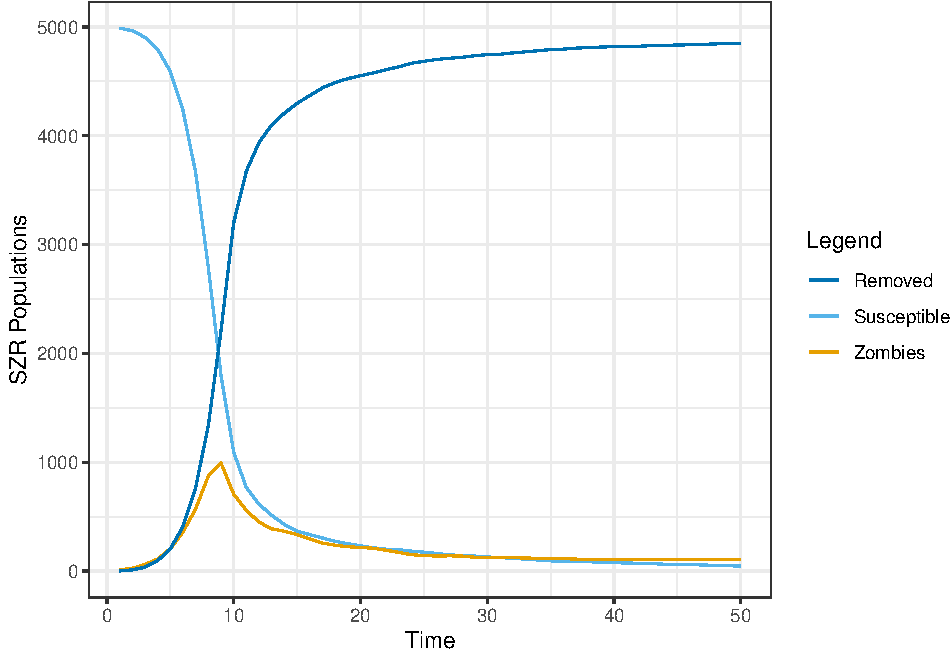
\includegraphics[width=0.6\linewidth]{SC2_Report_files/figure-latex/eval-1} \end{center}

\begin{Shaded}
\begin{Highlighting}[]
\NormalTok{simulated.mat }\OtherTok{\textless{}{-}}\NormalTok{ new.example}\SpecialCharTok{$}\NormalTok{results}
\NormalTok{simulated.mat  }\OtherTok{\textless{}{-}} \FunctionTok{as.matrix}\NormalTok{(simulated.mat[,}\DecValTok{2}\SpecialCharTok{:}\DecValTok{4}\NormalTok{])}
\FunctionTok{head}\NormalTok{(simulated.mat )}
\end{Highlighting}
\end{Shaded}

\begin{verbatim}
##       S.t Z.t R.t
## [1,] 4990  10   0
## [2,] 4966  24  10
## [3,] 4906  60  34
## [4,] 4796 110  94
## [5,] 4592 204 204
## [6,] 4234 358 408
\end{verbatim}

\begin{Shaded}
\begin{Highlighting}[]
\NormalTok{priorMin }\OtherTok{\textless{}{-}} \FunctionTok{c}\NormalTok{(}\FloatTok{0.000004}\NormalTok{,}\FloatTok{0.000004}\NormalTok{,  }\FloatTok{0.000004}\NormalTok{) }
\NormalTok{priorMax }\OtherTok{\textless{}{-}} \FunctionTok{c}\NormalTok{(}\FloatTok{0.0015}\NormalTok{ ,}\FloatTok{0.001}\NormalTok{, }\FloatTok{0.001}\NormalTok{)}
\NormalTok{res }\OtherTok{\textless{}{-}} \FunctionTok{abcRej}\NormalTok{(simulated.mat , }\DecValTok{10000}\NormalTok{, }\DecValTok{400}\NormalTok{, priorMin, priorMax)}
\FunctionTok{head}\NormalTok{(res)}
\end{Highlighting}
\end{Shaded}

\begin{verbatim}
##              [,1]         [,2]         [,3]
## [1,] 0.0004250723 0.0008617067 0.0006589291
## [2,] 0.0004237616 0.0009770686 0.0007613837
## [3,] 0.0003875616 0.0004843493 0.0006826764
## [4,] 0.0003708313 0.0006252518 0.0007569413
## [5,] 0.0004010205 0.0007269969 0.0005887166
## [6,] 0.0004492728 0.0009563075 0.0002842800
\end{verbatim}

\begin{Shaded}
\begin{Highlighting}[]
\FunctionTok{library}\NormalTok{(latex2exp)}
\FunctionTok{require}\NormalTok{(ggplot2)}
\FunctionTok{require}\NormalTok{(gridExtra)}
\NormalTok{plot.posterior.samples }\OtherTok{\textless{}{-}} \ControlFlowTok{function}\NormalTok{(sample, mean)\{}
\NormalTok{  beta\_plot }\OtherTok{\textless{}{-}} \FunctionTok{ggplot}\NormalTok{(}\AttributeTok{data =}\NormalTok{ sample, }\FunctionTok{aes}\NormalTok{(}\AttributeTok{x =}\NormalTok{ beta)) }\SpecialCharTok{+} 
    \FunctionTok{geom\_density}\NormalTok{(}\AttributeTok{colour =} \StringTok{"steelblue2"}\NormalTok{, }\AttributeTok{fill =} \StringTok{"steelblue2"}\NormalTok{, }\AttributeTok{alpha =} \FloatTok{0.5}\NormalTok{) }\SpecialCharTok{+}
    \FunctionTok{geom\_vline}\NormalTok{(}\FunctionTok{aes}\NormalTok{(}\AttributeTok{xintercept =}\NormalTok{ mean[}\DecValTok{1}\NormalTok{]))}\SpecialCharTok{+}
    \FunctionTok{labs}\NormalTok{(}\AttributeTok{x =} \FunctionTok{TeX}\NormalTok{(}\StringTok{"$}\SpecialCharTok{\textbackslash{}\textbackslash{}}\StringTok{hat\{}\SpecialCharTok{\textbackslash{}\textbackslash{}}\StringTok{beta\}$"}\NormalTok{), }\AttributeTok{y =} \StringTok{"Accepted Samples"}\NormalTok{) }\SpecialCharTok{+}
    \FunctionTok{theme\_classic}\NormalTok{()}
\NormalTok{  kappa\_plot }\OtherTok{\textless{}{-}} \FunctionTok{ggplot}\NormalTok{(}\AttributeTok{data =}\NormalTok{ sample, }\FunctionTok{aes}\NormalTok{(}\AttributeTok{x =}\NormalTok{ kappa)) }\SpecialCharTok{+} 
    \FunctionTok{geom\_density}\NormalTok{(}\AttributeTok{fill =} \StringTok{"steelblue2"}\NormalTok{, }\AttributeTok{alpha =} \FloatTok{0.5}\NormalTok{,}\AttributeTok{colour =} \StringTok{"steelblue2"}\NormalTok{) }\SpecialCharTok{+}
    \FunctionTok{geom\_vline}\NormalTok{(}\FunctionTok{aes}\NormalTok{(}\AttributeTok{xintercept =}\NormalTok{ mean[}\DecValTok{2}\NormalTok{])) }\SpecialCharTok{+}
    \FunctionTok{labs}\NormalTok{(}\AttributeTok{x =} \FunctionTok{TeX}\NormalTok{(}\StringTok{"$}\SpecialCharTok{\textbackslash{}\textbackslash{}}\StringTok{hat\{}\SpecialCharTok{\textbackslash{}\textbackslash{}}\StringTok{kappa\}$"}\NormalTok{), }\AttributeTok{y =} \StringTok{"Accepted Samples"}\NormalTok{) }\SpecialCharTok{+}
    \FunctionTok{theme\_classic}\NormalTok{()}
\NormalTok{  rho\_plot }\OtherTok{\textless{}{-}} \FunctionTok{ggplot}\NormalTok{(}\AttributeTok{data =}\NormalTok{ sample, }\FunctionTok{aes}\NormalTok{(}\AttributeTok{x =}\NormalTok{ rho)) }\SpecialCharTok{+} 
    \FunctionTok{geom\_density}\NormalTok{(}\AttributeTok{colour =} \StringTok{"steelblue2"}\NormalTok{, }\AttributeTok{fill =} \StringTok{"steelblue2"}\NormalTok{, }\AttributeTok{alpha =} \FloatTok{0.5}\NormalTok{) }\SpecialCharTok{+}
    \FunctionTok{geom\_vline}\NormalTok{(}\FunctionTok{aes}\NormalTok{(}\AttributeTok{xintercept =}\NormalTok{ mean[}\DecValTok{3}\NormalTok{]))}\SpecialCharTok{+}
    \FunctionTok{labs}\NormalTok{(}\AttributeTok{x =} \FunctionTok{TeX}\NormalTok{(}\StringTok{"$}\SpecialCharTok{\textbackslash{}\textbackslash{}}\StringTok{hat\{}\SpecialCharTok{\textbackslash{}\textbackslash{}}\StringTok{rho\}$"}\NormalTok{), }\AttributeTok{y =} \StringTok{"Accepted Samples"}\NormalTok{) }\SpecialCharTok{+}
    \FunctionTok{theme\_classic}\NormalTok{()}
  \FunctionTok{return}\NormalTok{(}\FunctionTok{list}\NormalTok{(beta\_plot, kappa\_plot, rho\_plot))}
\NormalTok{\}}
\end{Highlighting}
\end{Shaded}

\begin{Shaded}
\begin{Highlighting}[]
\FunctionTok{library}\NormalTok{(ggplot2)}
\FunctionTok{library}\NormalTok{(dplyr)}
\FunctionTok{library}\NormalTok{(ggthemes)}
\NormalTok{means }\OtherTok{\textless{}{-}} \FunctionTok{c}\NormalTok{(new.example}\SpecialCharTok{$}\NormalTok{beta, new.example}\SpecialCharTok{$}\NormalTok{kappa, new.example}\SpecialCharTok{$}\NormalTok{rho)}
\NormalTok{samples }\OtherTok{\textless{}{-}}\NormalTok{ res }\SpecialCharTok{\%\textgreater{}\%}
  \FunctionTok{as\_tibble}\NormalTok{()}
\FunctionTok{colnames}\NormalTok{(samples) }\OtherTok{\textless{}{-}} \FunctionTok{c}\NormalTok{(}\StringTok{"beta"}\NormalTok{, }\StringTok{"kappa"}\NormalTok{, }\StringTok{"rho"}\NormalTok{)  }

\NormalTok{plots }\OtherTok{\textless{}{-}} \FunctionTok{plot.posterior.samples}\NormalTok{(samples, means)}
\NormalTok{plots[[}\DecValTok{1}\NormalTok{]]}
\end{Highlighting}
\end{Shaded}

\begin{center}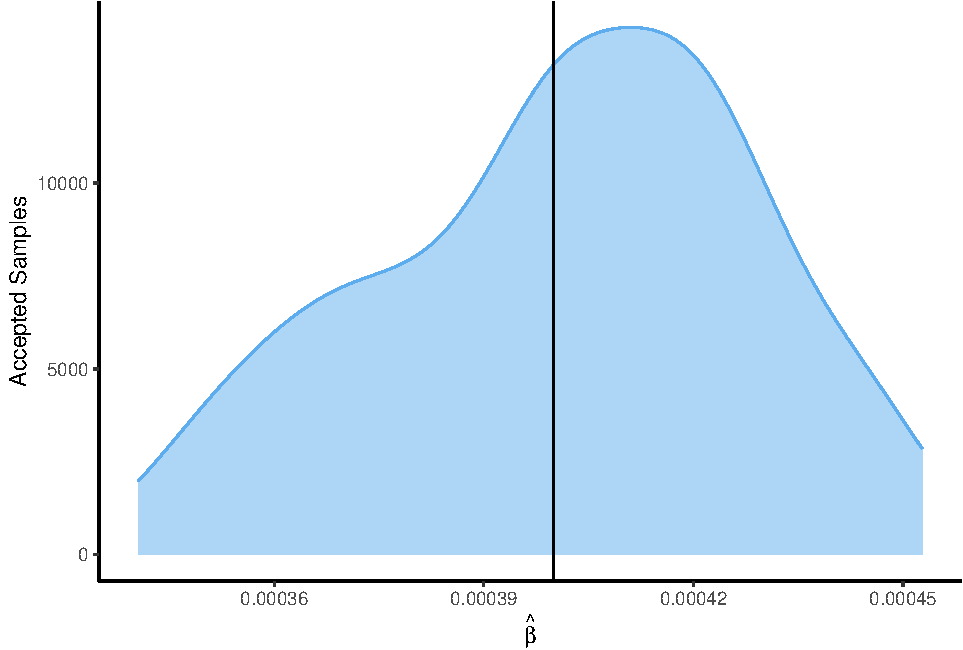
\includegraphics[width=0.6\linewidth]{SC2_Report_files/figure-latex/unnamed-chunk-4-1} \end{center}

\begin{Shaded}
\begin{Highlighting}[]
\NormalTok{plots[[}\DecValTok{2}\NormalTok{]]}
\end{Highlighting}
\end{Shaded}

\begin{center}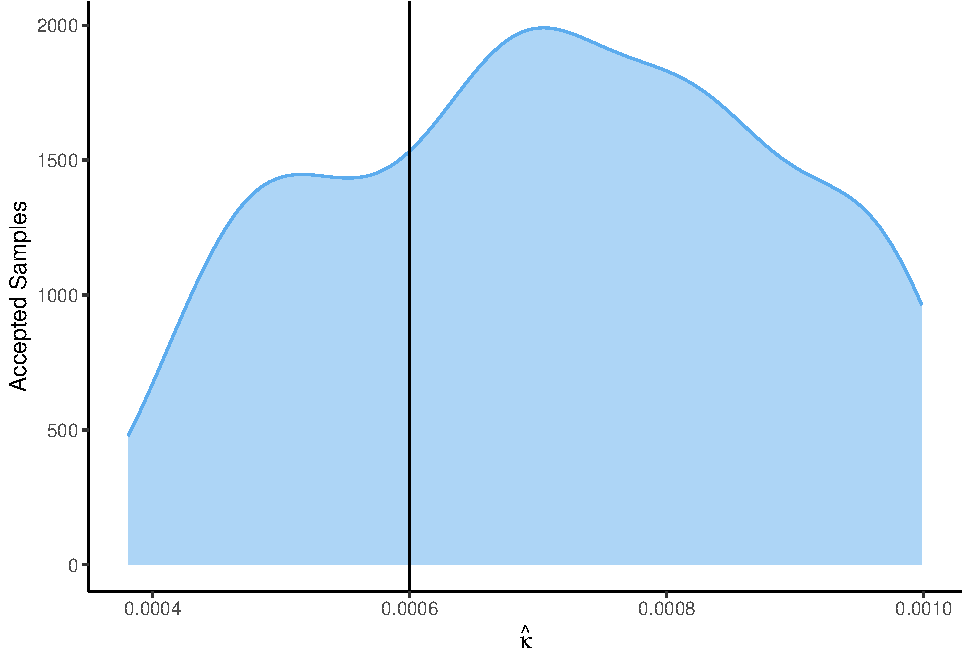
\includegraphics[width=0.6\linewidth]{SC2_Report_files/figure-latex/unnamed-chunk-4-2} \end{center}

\begin{Shaded}
\begin{Highlighting}[]
\NormalTok{plots[[}\DecValTok{3}\NormalTok{]]}
\end{Highlighting}
\end{Shaded}

\begin{center}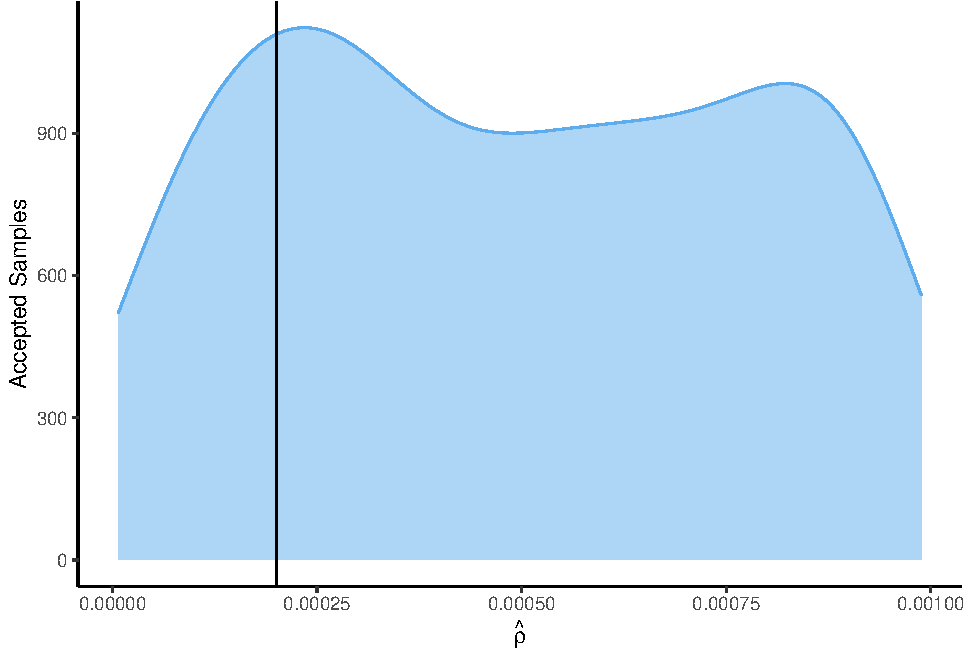
\includegraphics[width=0.6\linewidth]{SC2_Report_files/figure-latex/unnamed-chunk-4-3} \end{center}

\end{document}
